%!TEX root = ../main.tex

% \part{Grundlagen}
% \chapter{Kombinatorik}
\paragraph{Mit Zurücklegen, mit Betrachtung der Reihenfolge}
$n$ Möglichkeiten pro Zug, $n^k$ insgesamt

\paragraph{Ohne Zurücklegen, mit Betrachtung der Reihenfolge}
1. Zug, $n$ Möglichkeiten, 2. Zug, $n-1$ Mögl. k. Zug, $n-k+1$ Möglichkeiten.

$n=\frac{n!}{(n-k)!}=n^{\underline k}$

\paragraph{Ohne Zurücklegen, ohne Betrachtung der Reihenfolge}
Jede Kombination v.O. erlaubt $k!$ Anordnungen, aus k Zahlen k mal Ziehen ohne Zurücklegen ohne Reihenfolge, $k^{\underline k}=k!$.

Also $\frac{n^{\underline k}}{k!}=\frac{n!}{k!*(n-k)!}=\binom nk$

\paragraph{Mit Zurücklegen, ohne Betrachtung der Reihenfolge}


\part{Statistik}
% \chapter{Themenbereiche}
% \section{Desktriptive Statistik}

% \section{Explorative Statistik}

% \section{Induktive Statistik}





\chapter{Grundbegriffe}
\section{Grundbegriffe der Statistik}
\begin{description}
	\item[Statistische Einheit]
	Objekte die erfasst werden und an denen die interessierenden Größen erfasst werden

	\item[Grundgesamtheit]
	Menge aller für die Fragestellung relevanten statistischen Einheiten

	\item[Teilgesamtheit]
	Teilmenge der Grundgesamtheit

	\item[Stichprobe]
	Tatsächlich untersuchte Teilmenge der Grundgesamtheit

	\item[Merkmal, Variable]
	Größe von Interesse

	\item[Merkmalsausprägung, Wert]
	Konkreter Wert des Merkmals für eine bestimmte statistische Einheit
\end{description}

\section{Charakterisierung der Merkmale}
\begin{description}
	\item[diskret]
	Merkmale, die nur endlich viele oder abzählbar unendlich viele Ausprägungen annehmen sind diskret.
	\item[stetig]
	Merkmale, die Werte aus einem Intervall annehmen können heißen stetig.
	\item[quasi-stetig]
	Merkmale, die sich nur diskret messen lassen aber aufgrund einer sehr feinen Abstufung wie stetige Merkamle behandelt werden können.
\end{description}

Die Ausprägungen eines stetigen Merkmals lassen sich immer so zusammenfassen, dass es als diskret angesehen werden kann. Die Ausprägungen heißen dann gruppiert oder klassiert.



\section{Skalen}
Zusätzlich zur Charakterisierung der Merkmale werden diese anhand ihres Skalenniveaus unterschieden.
\begin{description}
	\item[Nominalskala]
		Wenn die Ausprägungen Namen oder Kategorien sind, die den Einheiten zugeordnet werden heißt das Merkmal \emph{nominalskaliert}. Beispielsweise Geschlecht oder Verwendungszweck.
	\item[Ordinalskala]
		Merkmale mit Ausprägungen zwar mit Ordnung, bei denen allerdings ein Abstand der Merkamale nicht interpretier- oder vergleichbar ist heißen \emph{ordinalskaiert}. Ein Beispiel hierfür wären Schulnoten.
	\item[Kardinalskala]
		Ein kardinalskaliertes Merkmal wird oft auch metrisch bezeichnet. Hierbei sind die Abstände der Ausprägungen interpretierbar und zusätzlich ist ein sinnvoller Nullpunkt der Skala festgelegt oder bestimmbar.
\end{description}

Auf Basis dieser Skalenmerkmale nennt man Merkmale mit endlich vielen Ausprägungen, die höchstens ordinalskaliert sind \emph{qualitative} oder \emph{kategoriale Merkmale}. Diese geben eine Qualität aber nicht ein Ausmaß wieder. 

Geben die Ausprägungen jedoch eine Intensität oder Ausmaß wieder so spricht man von \emph{quantitativen Merkmalen}. Alle Messungen mit Zahlenwerten stellen Ausprägungen quantiativer Merkmale dar. Ein kardinalskaliertes Merkmal ist stets quantitativ.

% \section{Datengewinnung, Datenerhebung}
% S.18 ff



\chapter{Verteilungen und ihre Darstellungen}
\section{Häufigkeiten}
Als \emph{Urliste} bezeichnet man die Menge der Merkmale $X$ der Untersuchungseinheiten $U=\simpleset{x_1,\ldots,x_n}$.

Die \emph{auftretenden Ausprägungen} von $X$ sind die Werte $\simpleset{a_1,\ldots,x_n}\subseteq\simpleset{x_1,\ldots,x_n}, k\leq n$.
Oftmals treten in einem großen Datensatz der Größe $n$ nicht auch $n$ verschiedene Werte $x_i$ auf.

Damit definieren sich 
\begin{definition}{Absolute Häufigkeit}
	Die absolute Häufigkeit einer auftretenden Ausprägung $a$ in einer Urliste $U$ ist
	\begin{equation*}
		h(a)=\left|\set{i\in\N}{x_i=a, x_i\in U}\right|.
	\end{equation*}
\end{definition}
Es gilt immer, dass die Summe aller absoluten Häufigkeiten gleich der Datensatzgröße ist
\begin{equation*}
	\sum\limits_{i=1}^n h(a_i)=|U|.
\end{equation*}

Die absolute Häufigkeitsverteilung ist dargestellt durch die Folge von Werten
$$h_1,\ldots,h_k=h(a_i),\ldots,h(a_k)$$

\begin{definition}{Relative Häufigkeit}
	Die relative Häufigkeit einer auftretenden Ausprägung $a$ in einer Urliste $U$ ist
	\begin{equation*}
		f(a)=\frac{h(a)}{|U|}.
	\end{equation*}
\end{definition}
Es gilt ähnlich wie bei der absoluten Häufigkeit für die Summe
\begin{equation*}
	\sum\limits_{i=1}^n f(a_i)=1.
\end{equation*}


Eine grafische Darstellung einer Häufigkeitsverteilung nennt man ein \emph{Histogramm}. Bei Histogrammen ist auf die Flächentreue zu achten, das bedeutet, dass der Flächeninhalt der aufgetragenen Rechtecke proportional (oder gleich) zu $h_j$ oder $f_j$ ist. So kann das menschliche Auge die Verteilung besser wahrnehmen.

Hat das Histogramm einer Verteilung nur einen deutlich erkennbaren Hochpunkt (Gipfel), heißt sie \emph{unimodal}. Treten mehrere Gipfel auf nennt man die Verteilung \emph{multimodal}. Bei zwei Gipfeln spricht man von einer \emph{bimodalen} Verteilung.

Man nennt eine Verteilung \emph{symmetrisch}, wenn es eine Symmetrieachse gibt, sodass die rechte und linke Hälfte der Verteilung annähernd zueinander spiegelbildlich sind. 
Eine Verteilung heißt \emph{schief}, wenn sie deutlich unsymmetrisch ist. Sie heißt dann \emph{linkssteil oder rechtsschief}, wenn der überwiegende Anteil von Daten linksseitig konzentriert ist. Dann steigt die Verteilung links deutlich steiler ab als rechts. Entsprechend \emph{rechtssteile oder linksschiefe} Verteilungen.


\section{Kumulierte Häufigkeiten}
Die kumulierten Häufigkeitsverteilungen geben an, wie viele Datenpunkte der Urliste, beziehungsweise welcher Anteil der Daten unterhalb einer Schranke liegen. Um diese Aussage sinnvoll zu beantworten ist zumindest eine Ordinalskala nötig.

\begin{definition}{Absolute kumulierte Häufigkeitsverteilung}
	Die absolut kumulierte Häufigkeitsverteilung ist die Funktion
	\begin{equation*}
		H(x)=\sum\limits_{i:a_i\leq x} h_i.
	\end{equation*}
\end{definition}
\begin{definition}{Relative kumulierte Häufigkeitsverteilung}
	Die relative kumulierte Häufigkeitsverteilung oder auch empirische Verteilungsfunktion ist
	\begin{equation*}
		F(x)=\sum\limits_{i:a_i\leq x} f_i.
	\end{equation*}
\end{definition}
Die kumulierten Häufigkeitsverteilungen sind monoton wachsende Treppenfunktionen, die an den Sprungstellen rechtsseitig stetig sind.



\section{Gruppierung}
Sind alle auftretenden Ausprägungen Elemente eines Interfalls $[a,b]$, lässt sich dieses in gleich große Klassen der Größe $d$ unterteilen.

Eine Klassifizierung ist allgemein
\begin{equation*}
	[a, c_1), \ldots, [c_i,c_{i+1}), [c_{i+1},c_{i+2}), \ldots\quad \forall i: c_{i+1}-c_i=d
\end{equation*}

Klassifizierte Daten sind i.A. einfacher zu interpretieren als große Mengen von Daten, die sich nur wenig voneinander unterscheiden.

Der maximale Fehler bei der Klassifizierung ist die halbe Klassengröße.





\section{Lagemaße}
Lagemaße helfen beim Vergleich verschiedener Eigenschaften, bzw dem Vergleich verschiedener statistischer Einheiten mit einer gemeinsamen Eigenschaft. 

\begin{definition}{Lagemaß}
	Ein \emph{Lagemaß} ist eine Abbildung $L:\R^n\rightarrow \R$ mit der Eigenschaft
	\begin{equation*}
		L(x_1+a,\ldots,x_n+a)=L(x_1,\ldots,x_n)+a\quad \forall a,x_i\in\R\enspace (1\leq i\leq n)
	\end{equation*}
	Ein Lagemaß beschreibt das Zentrum einer Verteilung.
\end{definition}

Beispiele für Lagemaße sind

\subsection{Arithmetisches Mittel}
Das arithmetische Mittel ist nur für quantitative Merkmale sinnvoll. Es berechnet sich durch
\begin{equation*}
    \overline x=\frac 1n \sum\limits_{i=1}^n x_i=\sum\limits_{i=1}^n (a_i*f_i)
\end{equation*}
aus Rohdaten beziehungsweise aus den Häufigkeitsdaten.

Mit dem arithmetischen Mittel gilt die sogenannte \emph{Schwerpunkteigenschaft}
\begin{equation*}
	\sum\limits_{i=1}^n(x_i-\overline x)=0.
\end{equation*}

Unter einer linearen Transformation $x\mapsto ax+b$ verhält sich das arithmetische Mittel analog
\begin{equation*}
    \overline x =\frac 1n\sum_{i=1}^n (ax_i+b)=\frac an\sum_{i=1}^n x_i+b=a\overline x +b
\end{equation*}


Wie aus der Formel erkennbar, ist das arithmetische Mittel extrem empfindlich gegen Ausreißer. Dafür wurden die folgenden Mittel eingeführt.

\paragraph{Das getrimmte Mittel}
Um Ausreißer weniger stark ins Gewicht fallen zu lassen wird der Datensatz absichtlich verkleinert. Beim getrimmten Mittel aus einer sortiert vorliegenden Liste von Daten werden zum Beispiel die oberen und unteren $5\%$ der Daten abgeschnitten, damit fallen auch eventuelle Ausreißer raus. Die Datensatzgröße bleibt jedoch nicht erhalten.

\paragraph{Das winsorisierte Mittel}
Ähnlich wie beim getrimmten Mittel wird der Datensatz beim winsorisierten Mittel von oben und unten herein bearbeitet. Anstatt Daten zu löschen werden beispielsweise die oberen $5\%$ durch den nächstkleineren Wert ersetzt. Hierbei bleibt also die Datensatzgröße gleich.

\subsection{Median}
Der Median stellt ein robusteres Lagemaß als das arithmetische Mittel dar, er ist resistenter gegen Ausreißer im Datensatz.
Für $x_1\leq x_2\leq\ldots\leq x_n$, also einen sortiert vorliegenden Datensatz ist der Median
\begin{equation*}
	x_{\operatorname{med}}=
	\begin{cases}
		x_{\frac{n+1}2}& \text{$n$ ungerade}\\
		\frac 12 (x_{\frac n2}+x_{\frac n2 +1})& \text{$n$ gerade}\\
	\end{cases}
\end{equation*}
Benötigt eine Zahlenordnung, also eine Ordinalskala.

Der Modus verhält sich unter linearer Transformation $y=ax+b$ genauso wie das arithmetische Mittel $y_{\operatorname{med}}=ax_{\operatorname{med}}+b$.

Mindestens $50\%$ der Daten sind kleiner oder gleich $x_{\operatorname{med}}$, genauso sind mindestens $50\%$ der Daten größer oder gleich dem Median $x_{\operatorname{med}}$.

\subsection{Modus}
Der Modus ist die Ausprägung größter Häufigkeit $x_{\operatorname{mod}}=a_i$ mit $h(a_i)=\max \set{h(a)}{a\in A}$ wobei $A$ die Menge aller vorkommenden Ausprägungen der Urliste ist.
Der Modus ist dann eindeutig, wenn die Häufigkeitsverteilung ein eindeutiges Maximum besitzt.

Der Modus empfiehlt sich schon für nominalskalierte Daten.

Der Modus verhält sich unter linearer Transformation $y=ax+b$ genauso wie das arithmetische Mittel $y_{\operatorname{mod}}=ax_{\operatorname{mod}}+b$.



\subsection{Geometrisches Mittel}
Für eine Urliste $U=\simpleset{u_1,\ldots,u_n}$ ist das geometrische Mittel definiert als
\begin{equation*}
	x_{\operatorname{geom}}=\sqrt[n]{\prod_{i=1}^n u_i}.
\end{equation*}
Das geometrische Mittel wird z.B. bei der Berechnung des effektiven Jahreszinses verwendet, es stellt jedoch kein Lagemaß im engeren Sinne dar.

\subsection{Harmonisches Mittel}
Für eine Urliste $U=\simpleset{u_1,\ldots,u_n}$ ist das harmonische Mittel definiert als
\begin{equation*}
	x_{\operatorname{harm}}=\frac{1}{\frac 1n\sum_{i=1}^n \frac 1{x_i}}.
\end{equation*}
Genauso wie das geometrische Mittel zählt das harmonische nicht zu den Lagemaßen im engeren Sinne.



\section{Lageregeln}
Für symmetrische Verteilungen gilt $\overline x\approx x_{\operatorname{med}}\approx x_{\operatorname{mod}}$.

Für linkssteile Verteilungen $\overline x> x_{\operatorname{med}}> x_{\operatorname{mod}}$.

Und ebenso für rechtssteile Verteilungen $\overline x< x_{\operatorname{med}}< x_{\operatorname{mod}}$.

\section{Streuungsmaße}
Um eine Verteilung sinnvoll beschreiben zu können sind zusätzlich zu den Lagemaßen noch Aussagen über die Streuung der Daten um das Mittel nötig.

\begin{definition}{Streuungsmaß}
	Ein \emph{Streuungsmaß} ist eine Abbildung $S:\R^n\rightarrow \R$ für die gilt
	\begin{equation*}
		S(x_1+a,\ldots,x_n+a)=S(x_1,\ldots,x_n) \quad\forall a,x_i\in\R (1\leq i\leq n)
	\end{equation*}
	Ein Streuungsmaß stellt dar, wie weit gestreut Werte einer Verteilung um ein Mittel liegen.
\end{definition}

\subsection{Variationsbreite, Stichprobenspannweite}
Die Stichproblenspannweite stellt dar, in welchem Bereich die Ausprägungen liegen, denn diese ist einfach
\begin{equation*}
	x_{\operatorname{max}}-x_{\operatorname{min}}.
\end{equation*}

\subsection{Standardabweichung}
Die Standardabweichung ist für eine Urliste $U=\simpleset{x_1,\ldots,x_n}$ von metrischen Daten definiert als
\begin{equation*}
	\tilde s=\sqrt{\frac 1n\sum_{i=1}^n (x_i-\overline x)^2}=\sqrt{\sum_{i=1}^n (a_i-\overline x)^2*f_i}
\end{equation*}
wobei die $a_i$ die Ausprägungen der Urliste sind und $f_i$ die relative Häufigkeit der Ausprägung $a_i$ ist.

Unter einer linearen Transformation $x\mapsto ax+b$ der Ausprägungen wird $\tilde s$ um $|a|$ gedehnt. Eine Verschiebung der Werte um $b$ hat keine Auswirkung.

\subsection{Variationskoeffizient}
Der Variationskoeffizient ist eine maßstabsunabhängige Maßzahl für die Streuung, sie basiert auf der Standardabweichung und ist definiert als
\begin{equation*}
	v=\frac{\tilde s}{\overline x},\quad \overline x>0
\end{equation*}

\subsection{Varianz, empirische Varianz}
Die empirische Varianz ist das Quadrat der Standardabweichung $\tilde s^2$.

\subsection{Stichprobenvarianz}
Die Stichprobenvarianz stellt ein nicht resistentes Streuungsmaß dar. Sie ist für eine Urliste $U=\simpleset{x_1,\ldots,x_n}$ definiert als
\begin{equation*}
	s^2=\frac{1}{n-1}\sum_{i=1}^n (x_i-\overline x)^2=\frac{1}{n-1}\sum_{i=1}^n x_i^2 - n*\overline x^2
\end{equation*}

\subsection{Mittlere absolute Abweichung vom Median}
Die mittlere absolute Abweichung vom Median stellt eine robustere Alternative zur Stichprobenvarianz dar. Sie ist für eine Urliste $U=\simpleset{x_1,\ldots,x_n}$ definiert als 
\begin{equation*}
	\frac 1n\sum_{i=1}^n|x_i-x_{\operatorname{med}}|
\end{equation*}


\subsection{Quantile}
Ein Quantil ist eine Kennzahl, die Daten nach einer relativen Häufigkeit trennt. So trennt das $p$-Quantil einer Verteilung die Daten som dass etwa $p*100\%$ der Daten darunter und $(1-p)*100\%$ darüber liegen. Damit ist der Median gerade das $50\%$-Quantil.

\begin{definition}{Quantile}
	Sei $U=\simpleset{x_1,\ldots,x_n}$ eine geordnete Urliste, d.h. $x_1\leq\ldots\leq x_j\leq\ldots\leq x_n$. Das $p$-Quantil $x_p$ ist eine Ausprägung $x_p\in U$ für die gilt
	\begin{equation*}
		\frac{\left|\set{i\in\N}{x_i\leq x_p, x_i\in U}\right|}{n}\geq p \text{ und } \frac{\left|\set{i\in\N}{x_i\geq x_p, x_i\in U}\right|}{n}\geq 1-p
	\end{equation*}
	Das heißt es liegen $p\%$ der Daten unterhalb und $(1-p)\%$ der Daten oberhalb des $p$-Quantils.

	Sinnvoll berechnen lässt sich das $p$-Quantil durch die Formel
	\begin{equation*}
		x_p=\begin{cases}
			\frac12(x_{(n*p)}+x_{(n*p+1)}) &\text{, falls $n*p$ ganzzahlig}\\
			x_{(\lfloor n*p\rfloor)+1} &\text{ sonst}
		\end{cases}
	\end{equation*}
\end{definition}
Dabei nennt man das $25\%$-Quantil auch das \emph{untere Quartil} und entsprechend das $75\%$-Quantil das \emph{obere Quartil}.

\begin{definition}{Interquartilsabstand}
	Für metrische Merkamel ist der sogenannte \emph{Interquartilsabstand (interquartile range)} die Distanz
	\begin{equation*}
		d_Q=\operatorname{IQR}=x_{0.75}-x_{0.25}.
	\end{equation*}
	Der IQR wird zum Beispiel beim Box-Plot verwendet. 
\end{definition}
Mit dem IQR können Zäune festgelegt werden, außerhalb derer sich höchstwahrscheinlich Ausreißer des Merkmals befinden. Ein Beispiel hierfür ist zum Beispiel der untere Zaun $z_u=x_{0.25}-1.5*d_Q$ und entsprechend die Obergrenze $z_o=x_{0.75}+1.5*d_q$, diese Werte werden wiederum beim Box-Plot verwendet.

\subsubsection{Box-Plot}
Das Box-Plot ist eine einfache Art und Weise die Ausprägungen einer Verteilung übersichtlich darzustellen. Für den Box-Plot ist ein 5-Tupel, $(z_u, x_{0.25}, x_{\operatorname{med}}, x_{0.75}, z_o)$ aus Werten ausreichend.
Beim Boxplot werden zwei Definitionen unterschieden, der \glqq normale\grqq\ Box-Plot und der modifizierte.

Beim Box-Plot wird ein Rechteck zwischen $x_{0.25}$ und $x_{0.75}$ gezeichnet, das $x_{\operatorname{med}}$ beinhaltet.
So sieht man dass sich 50\% der Datenpunkte innerhalb der Box befinden. Die nach außen gezeichneten Linien geben an, wie weit die Datenpunkte gestreut liegen. Diese sogenannten Whiskers enden bei $z_u$ bzw. $z_o$, diese Werte unterscheiden sich bei den beiden Definitionen.

\paragraph{Normaler Box-Plot}
Das Fünftupel besteht aus den Werten $(x_{\operatorname{min}}, x_{0.25}, x_{\operatorname{med}}, x_{0.75}, x_{\operatorname{max}})$. Wobei $x_{\operatorname{min}}$ und $x_{\operatorname{max}}$ die kleinste und größte Ausprägung der Verteilung darstellen. So sind alle Werte in der Spannweite der Whiskers enthalten. Ein Box-Plot sieht dann wie folgt aus

\begin{center}
	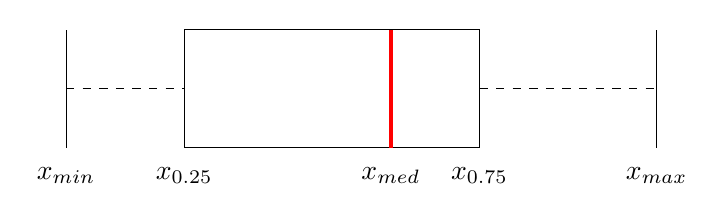
\begin{tikzpicture}[scale=0.75]
		\draw[black] (0,0) rectangle (5,2);
		\draw[black, dashed] (-2, 1) to (0,1) (5,1) to (8,1);
		\draw[black] (-2,0) to (-2,2) (8,0) to (8,2);
		\draw[red, line width=0.5mm] (3.5,0) to (3.5,2);

		\draw (-2,0) node[label={below:$x_{\operatorname{min}}$}] {};
		\draw (0,0) node[label={below:$x_{0.25}$}] {};
		\draw (3.5,0) node[label={below:$x_{\operatorname{med}}$}] {};
		\draw (5,0) node[label={below:$x_{0.75}$}] {};
		\draw (8,0) node[label={below:$x_{\operatorname{max}}$}] {};
	\end{tikzpicture}
\end{center}


\paragraph{Modifizierter Box-Plot (nach Fahrmeir)}
Der wichtigste Unterschied zum normalen Box-Plot ist dass, anstatt der minimalen und maximalen Werte für $z_u, z_o$ ein Zaun gewählt wurde. So ist $z_u=x_{0.25}-1.5*d_Q$ und $z_o=x_{0.75}+1.5*d_Q$ wobei $d_Q$ der Interquartilsabstand ist. Allerdings ist zu beachten dass die Whiskers von der größten/ kleinsten Ausprägung innerhalb des Zauns zur Box ausgehen. Liegen also beispielweise innerhalb des Bereichs $[z_u,x_{0.25}]$ keine Datenwerte, so existiert kein unterer Whisker. Datenpunkte, die außerhalb des Zauns liegen, werden mit Punkten dargestellt. Dies ist ein gutes Anzeichen für eventuelle Ausreißer.

\begin{center}
	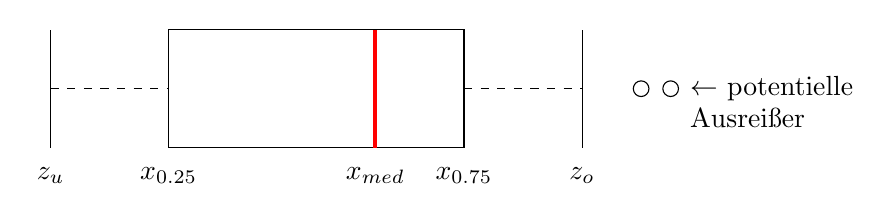
\begin{tikzpicture}[scale=0.75]
		\draw[black] (0,0) rectangle (5,2);
		\draw[black, dashed] (-2, 1) to (0,1) (5,1) to (7,1);
		\draw[black] (-2,0) to (-2,2) (7,0) to (7,2);
		\draw[red, line width=0.5mm] (3.5,0) to (3.5,2);

		\draw (-2,0) node[label={below:$z_u$}] {};
		\draw (0,0) node[label={below:$x_{0.25}$}] {};
		\draw (3.5,0) node[label={below:$x_{\operatorname{med}}$}] {};
		\draw (5,0) node[label={below:$x_{0.75}$}] {};
		\draw (7,0) node[label={below:$z_o$}] {};
		\draw (8,1) node[draw=black, fill=white, circle, inner sep=2pt] {};
		\draw (8.5,1) node[draw=black, fill=white, circle, inner sep=2pt] {};
		\draw (8.5,1) node[label={right:$\leftarrow$\ potentielle}] {};
		\draw (8.5,0.5) node[label={right:Ausreißer}] {};
	\end{tikzpicture}
\end{center}



\section{Schiefe und Wölbung}

\chapter{Multivariate}
Bisher wurden nur eindimensionale Daten erfasst, nicht aber verschschiedene Merkmale in Zusammenhang gebracht und gemeinsam betrachtet oder miteinander verglichen.
\section{Kontingenztafel}
Die Kontingenztabelle eignet sich zu Darstellung der gemeinsamen Verteilung von zwei Diskreten Merkmalen mit relativ wenigen Ausprägungen.

Auf Basis der Ausprägungen $a_1,\ldots,a_k$ des Merkmals $X$ und $b_1,\ldots,b_m$ für $Y$ liegen in der Urliste die gemeinsamen Messwerte vor. Das heißt die Urliste besteht aus den Tupeln $(a_i,b_j)$. Analog zum Eindimensionalen sind die absoluten Häufigkeiten $h_{ij}$ definiert. Darauf aufbauend ebenfalls völlig analog die relativen Häufigkeiten $f_{ij}$.

\paragraph{Kontingenztafel der absoluten Häufigkeiten}
Die aus diesen Werten entstehende Tafel heißt $(k\times m)$-Kontingenztafel der absoluten Häufigkeiten. Sie enthält neben den Häufigkeitsdaten zusätzlich noch die Spalten- beziehungsweise Zeilensummen der Werte.

\begin{center}
	\begin{tabular}{c|ccc|c}
		& $b_1$ & $\cdots$ & $b_m$ &\\
		\hline $a_1$ & $h_{11}$ & $\cdots$ & $h_{1m}$&$h_{1\cdot}=\sum_{i=1}^m h_{1i}$\\
		$a_2$ & $h_{21}$ & $\cdots$ & $h_{2m}$&$h_{2\cdot}=\sum_{i=1}^m h_{2i}$\\
		$\vdots$ & $\vdots$ & $\cdots$ & $\vdots$&\\
		$a_1$ & $h_{k1}$ & $\cdots$ & $h_{km}$&$h_{k\cdot}=\sum_{i=1}^m h_{ki}$\\
		\hline &$h_{\cdot1}$&&$h_{\cdot m}$&$n$
	\end{tabular}
\end{center}

Die Zeilensummen $h_{i\cdot}$ werden auch als Randhäufigkeiten des Merkmals $X$ bezeichnet. Diese Werte sind die einfachen Häufigkeiten mit denen das Merkmal $X$ die Werte $a_1,\ldots,a_k$ annimmt, wenn $Y$ nicht berücksichtigt wird.

Analog dazu sind die Spaltensummen die Häufigkeiten von $Y$ unter Vernachlässigung des Merkmals $X$.

\paragraph{Kontingenztafel der relativen Häufigkeiten}
Da Anteile beziehungsweise Prozente häufig anschaulicher sind als absolute Häufigkeitswerte betrachtet man häufig auch die Häufigkeitstafel der relativen Häufigkeiten. Diese entsteht durch teilen durch die Gesamtzahl $n$.

\begin{center}
	\begin{tabular}{c|ccc|c}
		& $b_1$ & $\cdots$ & $b_m$ &\\
		\hline $a_1$ & $h_{11}$ & $\cdots$ & $h_{1m}$&$f_{1\cdot}=\sum_{i=1}^m f_{1i}$\\
		$a_2$ & $f_{21}$ & $\cdots$ & $f_{2m}$&$f_{2\cdot}=\sum_{i=1}^m f_{2i}$\\
		$\vdots$ & $\vdots$ & $\cdots$ & $\vdots$&\\
		$a_1$ & $f_{k1}$ & $\cdots$ & $f_{km}$&$f_{k\cdot}=\sum_{i=1}^m f_{ki}$\\
		\hline &$f_{\cdot1}$&&$f_{\cdot m}$&$1$
	\end{tabular}
\end{center}

\section{Bedingte Häufigkeiten}
S125/110
\section{Darstellungen von Verteilungen}

\subsection{Lineare Regression}



\part{Stochastik}
%!TEX root = ../main.tex
\chapter{Wahrscheinlichkeitsräume}

\section{Allgemeine Definitionen}
\begin{itemize}
	\item Ein Wahrscheinlichkeitsraum besteht aus einem \emph{Grundraum} $\Omega$, einem System $\mathcal A$ von Teilmengen von $\Omega$ und der \emph{Wahrscheinlichkeitsverteilung} $P$.

	\item Der Grundraum $\Omega\neq \emptyset$ ist nichtleer und ist die Menge der Ergebnisse. Elemente $A\in\mathcal A$ heißen Ereignisse, ein Ereignis mit $|A|=1$ heißt Elementarereignis. Außerdem ist $\emptyset\in\mathcal A$ das \emph{unmögliche Ereignis} und $\Omega\in\mathcal A$ das sogenannte \emph{sichere Ereignis}.

	\item Die Wahrscheinlichkeitsverteilung ist eine Abbildung $P:\mathcal A\rightarrow \R$.

	\item Die Ereignismenge $\mathcal A$ muss unter den Mengenoperationen $\simpleset{\cap, \cup, \setminus}$ und Komplement abgeschlossen sein. Man nennt zwei Ereignisse $A, B\in\mathcal A$ \emph{unvereinbar}, wenn $A\cap B=\emptyset$ ($A$ und $B$ sind disjunkte Mengen). Für paarweise unvereinbare Ereignisse $A_i$ definieren wir $\bigcup_{i} A_i\coloneqq \sum_{i} A_i$.


	\item Eine \emph{Zufallsvariable} ist eine Abbildung $X:\Omega\rightarrow \R$, sie ordnet einem Ergebnis einen Wert zu. Zum Beispiel wäre die Augensumme beim Werfen mehrerer Würfel eine Zufallsvariable. Für eine Zufallsvariable $X$ sei $X^{-1}$ für eine beliebige Teilmenge $A\in\mathcal A$ definiert als das Urbild $X^{-1}(A)=\set{\omega\in\Omega}{X(\omega)\in A}$.
\end{itemize}


\paragraph{Kurzschreibweisen:}\label{Kurzschreibweisen1}
Für das Urbild eines Ereignisses bezüglich einer Zufallsvariable wird eine Kurzschreibweise definiert. So ist zum Beispiel $\simpleset{3\leq X\leq 4}\coloneqq X^{-1}([3,4])$. Auch eine Schreibweise wie $\simpleset{X=3}\cup\simpleset{X=4}\coloneqq X^{-1}(\simpleset{3,4})$ ist möglich.


\chapter{Diskrete Wahrscheinlichkeitsräume}
Einen einfachen Einstieg in die Wahrscheinlichkeitsräume stellen die endlichen Wahrscheinlichkeitsräume dar. Sie sind ein Sonderfall der diskreten Wahrscheinlichkeitsräume.
\section{Endliche Wahrscheinlichkeitsräume}
Ein Wahrscheinlichkeitsraum ist endlich, wenn $|\Omega|<\infty$ ist. Man verwendet dann üblicherweise $\mathcal A=\Pot(\Omega)$. Damit ist $\mathcal A$ unter allen Mengenoperationen abgeschlossen und für eine Zufallsvariable $X$ ist $X^{-1}(B)\in\mathcal A$ für alle $B\subseteq\R$.

\begin{definition}{Endlicher Wahrscheinlichkeitsraum}
	Das Paar $(\Omega, P)$ ist ein endlicher Wahrscheinlichkeitsraum, wenn gilt
	\begin{description}
		\item[\bf EW1] $\forall A\subseteq \Omega: P(A)\geq 0$
		\item[\bf EW2] $P(\Omega)=1$
		\item[\bf EW3] $\forall A,B\subseteq \Omega, A\cap B=\emptyset: P(A\cup B)\coloneqq P(A+B)=P(A)+P(B) $
	\end{description}
\end{definition}

\begin{satz}{Folgerungen aus der Definition}
	\begin{enumerate}
		\item $P(\emptyset)=0$
		\item $P\left(\sum_i A_i\right)=\sum_i P(A_i)$
		\item $0\leq P(A)\leq 1$
		\item $\forall A\subseteq\Omega: P(\bar A)=1-P(A)$
		\item $A\subseteq B\subseteq C\Rightarrow P(A)\leq P(B)$
		\item $\forall A,B\subseteq \Omega: P(A\cup B)=P(A)+P(B)-P(A\cap B)$
		\item $P\left(\bigcup_i A_i\right)\leq \sum_i P(A_i)$
		\item $P(A_1\cup A_2\cup A_3)=P(A_1)+P(A_2)+P(A_3)-P(A_1\cap A_2)-P(A_1\cap A_3)-P(A_2\cap A_3)+P(A_1\cap A_2\cap A_3)$
	\end{enumerate}
\end{satz}

\paragraph{Beispiel:}
Wir werfen einen Oktaeder, das heißt $\Omega=\simpleset{1,\ldots,8}$ und $\mathcal A=\Pot \Omega$. Es gilt $p(\omega)=P(\simpleset{\omega})=\frac 18$ für alle $\omega \in\Omega$. Wir definieren das Ereignis $A_1=\simpleset{2,3,5,7}$, also alle Primzahlen auf dem Würfel.
\begin{equation*}
	P(A_1)=p(2)+p(3)+p(5)+p(7)=\sum_{\omega\in A_1}p(\omega)=\frac12.
\end{equation*}
Analog ist für $A_2=\simpleset{1,3,5,7}$ die Wahrscheinlichkeit $P(A_2)=\frac12$. Für die Vereinigung gilt
\begin{equation*}
	P(A_1\cup A_2)=P(A_1)+P(A_2)-P(A_1\cap A_2)=\frac12+\frac12-\frac38=\frac58.
\end{equation*}

\subsection{Zufallsvariablen auf endlichen Wahrscheinlichkeitsräumen}
Zufallsvariablen auf endlichen Wahrscheinlichkeitsräumen sind dann Abbildungen $X:\Omega \rightarrow \R$ mit der Verteilung $P^X:\Pot(\Omega)\rightarrow \R$ wobei $P^X(B)\coloneqq P(X^{-1}(B))$ für alle $B\subseteq X(\Omega)$ ist.
\paragraph{Kurzschreibweisen:}
\begin{itemize}
	\item Völlig analog zu den bereits eingeführten \hyperref[Kurzschreibweisen1]{Kurzschreibweisen} definieren wir
		\begin{align*}
		    P^X(B)=P(X^{-1}(B))&=P(\set{\omega\in\Omega}{X(\omega)\in B})\\
		    &=P(\simpleset{X\in B})\\
		    &=P(X\in B)
		\end{align*}
	\item Darauf aufbauend ist $P(a\leq X\leq b)$ für $a,b\in\R$ die Wahrscheinlichkeit $P^X([a,b]\cap X(\Omega))$.
	\item Und für einelementige Mengen ist $P(X=x)=P(X\in \simpleset{x})$.
\end{itemize}

\begin{definition}{Verteilungsfunktion}
	Eine Verteilungsfunktion der Zufallsvariablen $X$ ist eine Abbildung $F^X:\R\rightarrow\R$ mit $F^X(x)=P(X\leq x)$. Dies ist eine monoton steigende, rechtsseitig stetige Funktion.
\end{definition}


\begin{definition}{Laplace-Experiment}
	Ein Laplace-Experiment entspricht der intuitiven Gleichverteilung. Es handelt sich um einen Wahrscheinlichkeitsraum $(\Omega,P)$ wobei $p(\omega)=\frac 1{|\Omega|}$ für alle $\omega\in\Omega$ gilt.
	
	Das bedeutet $\forall A\subseteq \Omega:P(A)=\frac{|A|}{|\Omega|}$.
\end{definition}
\paragraph{Bemerkung:}
Für eine Zufallsvariable $X$ ist $P^X$ in der Regel keine Gleichverteilung, da $|X^{-1}(\simpleset{\omega})|>1$ vorkommen kann.

\paragraph{Beispiel:}
Für zwei Würfel ist der Grundraum $\Omega=\simpleset{1,\ldots,6}^2$ und die Wahrscheinlichkeit der Elementarereignisse ist $p((\omega_1,\omega_2))=\frac{1}{36}$ für alle $(\omega_1,\omega_2)\in\Omega$. Die Zufallsvariable $M(\omega_1,\omega_2)=\max\simpleset{\omega_1,\omega_2}$ beschreibt das Maximum der beiden Würfelergebnisse. Damit ist 
\begin{equation*}
	\begin{array}{r|cccccc}
		m&1&2&3&4&5&6\\
		\hline P(M=m)&\sfrac{1}{36}&\sfrac{3}{36}&\sfrac{5}{36}&\sfrac{7}{36}&\sfrac{9}{36}&\sfrac{11}{36}
	\end{array}
\end{equation*}

\begin{definition}{Erwartungswert einer Zufallsvariablen}
	Der Erwartungswert einer Zufallsvariablen $X$ auf dem Wahrscheinlichkeitsraum $(\Omega,P)$ ist
	\begin{align*}
		E(X)&=\sum_{\omega\in\Omega} X(\omega)*P(\simpleset{\omega})\\
		&=\sum_{\mathclap{x\in X(\Omega)}}x*P(X=x)
	\end{align*}
\end{definition}

\begin{satz}{Sätze zum Erwartungswert}
	Für zwei Zufallsvariablen $X$ und $Y$ auf dem Wahrscheinlichkeitsraum $(\Omega,P)$ und $a\in\R$ gilt
	\begin{description}
		\item[Linearität 1] $E(X+Y)=E(X)+E(Y)$
		\item[Linearität 2] $E(a*X)=a*E(X)$
		\item[Indikatorfunktion] $E(1_A)=P(A)$ mit $1_A=1\Leftrightarrow X(\omega)\in A$
		\item[Ordnung] $\forall \omega\in\Omega: X(\omega)\leq Y(\omega) \Rightarrow E(X)\leq E(Y)$
	\end{description}
\end{satz}

\begin{definition}{Varianz und Standardabw. von Zufallsvariablen}
	Die Varianz einer Zufallsvariablen $X$ auf dem Wahrscheinlichkeitsraum $(\Omega,P)$ ist
	\begin{equation*}
		V(X)=E((X-E(X))^2).
	\end{equation*}
	Entsprechend zur Standardabweichung von Merkmalen aus der Statistik ist die Standardabweichung einer Zufallsvariablen die Wurzel der Varianz
	\begin{equation*}
		\sigma(X)=\sqrt{V(X)}.
	\end{equation*}
\end{definition}

\begin{satz}{Sätze zur Varianz}
	Für eine Zufallsvariable $X$ und alle $\alpha,\beta\in\R$ gilt für die Varianz
	\begin{enumerate}
		\item $V(\alpha X + \beta) = \alpha^2 V(X)$ (Lineare Transformation)
		\item $V(X)=E(X^2)-(E(X))^2$ (Verschiebungssatz)
		\item $V(X)\geq 0$
		\item $V(X)=0\Leftrightarrow   \exists!a\in\R: P(X=a)=1$
	\end{enumerate}
\end{satz}

\paragraph{Beweis:}
\begin{enumerate}
	\item Varianz einer linear transformierten Zufallsvariable
	\begin{align*}
		V(\alpha X + \beta)&=E[((\alpha X+\beta)-E(\alpha X+\beta))^2]\\
		&=E[((\alpha X)-\alpha E(X))^2] &\text{(Linearität)}\\
		&=E[\alpha^2(X-E(X))^2]\\ 
		&=\alpha^2E[X-E(X)^2]\\
		V(\alpha X + \beta)&=\alpha^2V(X)
	\end{align*}
	\item Beweis des sog. Verschiebungssatzes mit der Linearität des Erwartungswerts
	\begin{align*}
		V(X)&=E[(X-E(X))^2]\\
		&=E[X^2-2X*E(X)+E(X)^2]\\
		&=E(X^2)-2E(X)*E(E(X))+E(X)^2\\
		&=E(X^2)-E(X)^2\\
	\end{align*}
\end{enumerate}


\begin{satz}{Tschebyscheff-Ungleichung}
	\label{tschebyscheff}
	Für eine Zufallsvariable $X$ auf dem Wahrscheinlichkeitsraum $(\Omega,P)$ gilt für alle $\epsilon>0$
	\begin{equation*}
		P(|X-E(X)|\geq \epsilon)\leq \frac{V(X)}{\epsilon^2}
	\end{equation*}
\end{satz}

\begin{definition}{Bedingte Wahrscheinlichkeit}
	Auf Basis eines Zufallsexperiments wird die Wahrscheinlichkeit, dass ein Ereignis $B$ eintritt, während zusätzlich ein fest gewähltes Ereignis $A$ eintegtreten ist, \emph{bedingte Wahrscheinlichkeit} bezeichnet. Man interessiert sich also für die Wahrscheinlichkeit des Eregnisses $B$ unter der Bedingung, dass $A$ bereits eingetreten ist. In Zeichen ist die gesuchte Wahrscheinlichkeit
	\begin{equation*}
		P(B|A)=P_A(B)\coloneqq\frac{P(B\cap A)}{P(A)}
	\end{equation*}
\end{definition}

\subsection{Unabhängigkeit in endlichen Wahrscheinlichkeitsräumen}
\begin{definition}{Unabhängigkeit von Ereignissen}
	Man nennt zwei Ereignisse $A,B\subset \Omega$ \emph{unabhängig}, wenn
	\begin{equation*}
		P(A\cap B)=P(A)*P(B)
	\end{equation*}
	gilt.
\end{definition}
\paragraph{Bemerkung:}
\begin{itemize}
	\item Die Unabhängigkeit von Ereignissen ist offensichtlich eine symmetrische Relation.
	\item Unabhängigkeit ist nicht mit stochastischer Kausalität zu verwechseln
	\item Sind zwei Ereignisse unabhängig, dann ist die bedingte Wahrscheinlichkeit gleich der totalen
	\begin{equation*}
		P(A|B)=P(A).
	\end{equation*}
	\item Sind zwei Ereignisse $A,B$ unvereinbar, das heißt $A\cap B=\emptyset$, sind sie genau dann unabhängig, wenn $P(A)=0$ oder $P(B)=0$ gilt.
	\item Sind zwei Ereignisse $A,B$ unabhängig, so sind auch deren Komplemente $\overline A, \overline B$ unabhängig.
\end{itemize}


\begin{definition}{Unabhängigkeit von Zufallsvariablen}
	Zwei Zufallsvariablen in einem Wahrscheinlichkeitsraum $(\Omega,P)$ heißen sind unabhängig, wenn 
	für alle $B_X,B_Y\subseteq \Omega$ gilt
	\begin{align*}
		P(X\in B_X\wedge Y\in B_Y)&=P(X\in B_X)*P(Y\in B_Y)\\
		P(X^{-1}(B_X)\cap Y^{-1}(B_Y))&=P(X^{-1}(B_X))*P(Y^{-1}(B_Y))\\
	\end{align*}
\end{definition}
\paragraph{Bemerkung:}
Es reicht zwar diese Eigenschaft nur für die einelementigen Teilmengen von $\Omega$ zu zeigen, allerdings entstehen auch damit bereits zu viele Kombinationen.


\begin{satz}{Erwartungswert bei unabhängigen ZV}
	Für zwei unabhängige Zufallsvariablen gilt für das Produkt der beiden
	\begin{equation*}
		E(X*Y)=E(X)*E(Y)
	\end{equation*}
\end{satz}
\paragraph{Beweis:}
Für das Produkt zweier unabhängiger Zufallsvariablen ist der Erwartungswert
\begin{align*}
	E(X*Y)&=\sum_{\mathclap{z\in(X*Y)(\Omega)}}z*P(X*Y=z)\\
	&=\sum_{\mathclap{(x,y)\in X(\Omega)\times Y(\Omega)}}xy*P(X=x \wedge Y=x)\\
	&=\sum_{x\in X(\Omega)}\Big[x*P(X=x) * \sum_{\mathclap{y\in Y(\Omega)}} y*P(Y=y)\Big] &\text{(Unabhängigkeit)}\\
	&=\sum_{x\in X(\Omega)}x*P(X=x)* \sum_{\mathclap{y\in Y(\Omega)}} y*P(Y=y)\\
	&=E(X)*E(Y)
\end{align*}



%!TEX root = ../main.tex
\subsubsection{Binomialverteilung}
\begin{definition}{Bernoulli-Experiment}
	Ein Bernoulli-Experiment ist ein Zufallsexperiment mit genau zwei möglichen Ausgängen. Das heißt für eine Zufallsvariable $X$ gilt $X(\Omega)=\simpleset{0,1}$ mit den Wahrscheinlichkeiten
	\begin{align*}
		P(X=1)=p && P(X=0)=(1-p)=q
	\end{align*}
\end{definition}
\paragraph{Bemerkung:}
Der Erwartungswert eines Bernoulli-Experiments ist $E(X)=p$. Für die Varianz gilt 
\begin{equation*}
	V(X)=E(X)^2-2p*E(X)+p^2=p-p^2=p(1-p)=pq
\end{equation*}

Führt man nun $n$ \emph{unabhängige} Bernoulli-Experimente $X_i, i\in\simpleset{1,\ldots,n}$ durch, erhält man eine sogenannte \emph{Bernoulli-Kette} der Länge $n$. Ein Ereignis dieses Grundraums ist $\omega=(\omega_1,\ldots,\omega_n)$ wobei $X_i(\omega)=\omega_i$ gilt.

Der Grundraum der Bernoulli-Kette ist also $\Omega=\simpleset{0,1}^n$. Damit gilt für die Verteilung des Wahrscheinlichkeitsraums

\begin{align*}
	P(\simpleset{(\omega_1,\ldots,\omega_n)})&=P(X_1=\omega_1, X_2=\omega_2, \ldots, X_n=\omega_n)\\
	&=\prod_{i=1}^n P(X_i=\omega_i) &\text{(Unabhängigkeit)}\\
	&=\prod_{\mathclap{i:\omega_i=1}}p * \prod_{\mathclap{i:\omega_i=0}}(1-p)
\end{align*}
Damit ist bei $n$ Durchführungen die Wahrscheinlichkeit $k$ mal das Ergebnis $\omega_i=1$ zu erhalten ($k$ Treffer bei $n$ Versuchen) 
\begin{equation*}
	p^k*(1-p)^{n-k}
\end{equation*}

Betrachten wir nun also die Zufallsvariable $X$, die die Summe der Treffer beschreibt $X:\sum_{i=1}^n X_i$.
Das Ereignis $\simpleset{X=k}=\set{(\omega_1,\ldots,\omega_n)\in\Omega}{\sum_{i=1}^n \omega_i=k}$ beschreibt die Ausgänge, bei denen genau $k$ von $n$ Treffer aufgetreten sind. Es ist $|\simpleset{X=k}|=\binom nk$. Damit erhält man insgesamt
\begin{equation*}
	P(X=k)=\binom nk * p^k*(1-p)^{n-k}.
\end{equation*}
Man nennt $X$ dann \emph{binomialverteilt} mit den Parametern $n$ und $p$, man schreibt $X\sim Bin(n,p)$.

Für den Erwartungswert und die Varianz von binomialverteilten Zufallsvariablen gilt
\begin{align*}
	E(X)&=E\left(\sum_{i=1}^n X_i\right)\overset{\text{lin.}}=\sum_{i=1}^n E(X_i)=n*p\\
	V(X)&=V\left(\sum_{i=1}^n X_i\right)\overset{\text{unabh.}}=\sum_{i=1}^n V(X_i)=n*p(1-p)
\end{align*}
%!TEX root = ../main.tex
\subsubsection{Hypergeometrische Verteilung}
%!TEX root = ../main.tex
\subsection{Erweiterung auf allgemein diskrete Wahrscheinlichkeitsräume}
Bisher haben wir endliche Wahrscheinlichkeitsräume betrachtet, das heißt $0<|\Omega|<\infty$. Wir erlauben nun eine Erweiterung auf $0<|\Omega|\leq|\N|$.

\begin{definition}{Diskreter Wahrscheinlichkeitsraum}
	Das Paar $(\Omega, P)$ ist ein diskreter Wahrscheinlichkeitsraum, wenn
	\begin{description}
		\item[Nicht Negativität] $\forall A\subseteq \Omega: P(A)\geq 0$
		\item[Normiertheit] $P(\Omega)=1$
		\item[$\sigma$-Additivität] Für alle paarweise disjunkten $A_1,A_2,\ldots\subseteq \Omega $ gilt $P(\sum_{i=1}^\infty A_i)=\sum_{i=1}^\infty P(A_i)$ 
	\end{description}
	gilt.
\end{definition}

\paragraph{Konsequenzen aus der Erweiterung}
\begin{itemize}
	\item Endliche Wahrscheinlichkeitsräume sind Sonderfälle von diskreten Wahrscheinlichkeitsräumen.
	\item Es gilt wie im endlichen Fall $P(A)=\sum_{\omega\in A}P(\simpleset{\omega})$. Hier kann aber potentiell $A$ unendlich viele Elemente beinhalten, allerdings handelt es sich stets um eine absolut konvergente Reihe.
	\item Alle Rechenregeln für Wahrscheinlichkeiten gelten weiter.
	\item Aber $E(X)=\sum_{\omega\in\Omega}X(\omega)*P(\simpleset{\omega})$ ist eventuell eine nicht konvergente Reihe. Der Erwartungswert einer Zufallsvariable ist nur definiert, wenn $\sum_{\omega\in\Omega}|X(\omega)|*P(\simpleset{\omega})<\infty$.
\end{itemize}
\paragraph{Beispiel:}
Das sogenannte \emph{Sankt-Petersburg-Paradoxon} behandelt das Problem von nicht existierendem Erwartungswert.
Es wird eine Münze geworfen bis zum ersten Vorkommen von Zahl im Wurf $k$. Der Grundraum ist also $\Omega=\N$. Damit ist $P(\simpleset{k})=\frac{1}{2^k}$, die Zufallsvariable $X$ beschreibt die Auszahlung in Abhängigkeit von $k$, $X(k)=2^k{k-1}$.

Die Reihe
\begin{equation*}
	\sum_{k\in\N}X(k)*P(\simpleset{k})=\sum_{k=0}^\infty \frac12 \rightarrow \infty
\end{equation*}
ist divergent - der Erwartungswert $E(X)$ existiert nicht.

\subsubsection{Geometrische Verteilung}



\subsubsection{Poisson-Verteilung}
%!TEX root = ../main.tex
\subsection{Geometrische Verteilung}
Wir führen nun unabhängige Bernoulli-Experimente mit Trefferwahrscheinlichkeit $0<p<1$ so oft hintereinander aus, bis ein Erfolg eintritt. Damit ist der Grundraum die Menge
\begin{equation*}
	\Omega =\simpleset{\underset{\omega_1}{1},\underset{\omega_2}{01},\underset{\ldots}{001},0001,\ldots}.
\end{equation*}
$\Omega$ ist abzählbar unendlich groß. Aufgrund der Unabhängigkeit der einzelnen Experimente ist die Wahrscheinlichkeit für ein Ergebnis
\begin{equation*}
	P(\simpleset{\omega_k})=(1-p)^{k-1}*p=q^{k-1}p.
\end{equation*}

Die Zufallsvariable, die die Anzahl Misserfolge bis zum Erfolg zählt $X(\omega_k)=k-1$ heißt dann \emph{geometrisch verteilt} mit Parameter $p$, in Zeichen $X\sim \geom(p)$.

Es ist also
\begin{equation*}
	P(X=k)=q^kp.
\end{equation*}

Die Verteilungsfunktion an den Stellen $i\in \N$ der geometrisch verteilten Variable ist
\begin{equation*}
	F^X(i)=P(X\leq i) = \sum_{k=0}^i P(X=k)=p*\sum_{k=0}^i q^k=p*\frac{1-q^{i+1}}{1-q}=1-q^{i+1}.
\end{equation*}
Und analog gilt für den Erwartungswert
\begin{equation*}
 	E(X)=\sum_{i=0}^\infty i*P(X=i)=\sum_{i=0}^\infty i*q^ip=pq*\sum_{i=0}^\infty i*q^{i-1}\overset{\ref{eGeomZusatz}}=p*q*\frac1{(1-q)^2}=\frac{p*q}{p^2}=\frac qp=\frac1p-1
\end{equation*} 

Mit der Umformung
\begin{equation}
	\sum_{i=0}^\infty i*q^{i-1}=\sum_{i=0}^\infty \frac{\diff}{\diff q} q^k=\frac{\diff}{\diff q} \sum_{i=0}^\infty q^i = \frac{\diff}{\diff q}\frac{1}{1-q}=\frac{1}{(1-q)^2}.\label{eGeomZusatz}
\end{equation}

Die Varianz von $X$ ist dann
\begin{equation*}
	V(X)=\frac{1-p}{q^2}=\frac{q}{p^2}.
\end{equation*}


\paragraph{Beispiel:}
Wir betrachten ein Spiel mit Sammelbildern (z.B. Fußballspieler aus Hanuta). Die Zufallsvaraible $Y_i$ beschreibt die Anzahl Bilder, die man ziehen muss um seine Sammlung von $i$ Bildern auf $i+1$ zu vergrößern.

Damit ist die Anzahl an Misserfolgen vor dem richtigen Bild geometrisch verteilt
\begin{equation*}
	(Y_i-1)\sim \geom\Big(\frac{n-i}{n}\Big)\quad\Rightarrow E(Y_i)=E(Y_i-1)+1=\frac{1}{\frac{n-i}{n}}=\frac{n}{n-i}
\end{equation*}
Insgesamt beschreibt die Zufallsvariable $Y$ die benötigten Bilder für eine Sammlung der Größe $n$
\begin{equation*}
	Y=\sum_{i=0}^{n-1} Y_i\quad\Rightarrow E(Y)=\sum_{i=0}^{n-1} E(Y_i)=\sum_{i=0}^{n-1} \frac{n}{n-i}=n*\sum_{i=1}^{n}\frac1i\approx n*\ln(n)
\end{equation*}

Für maximal $63$ mögliche Bilder ist $E(Y)=297.88$ und die Näherung $63\ln(63)=261.01$.


\begin{satz}{Gedächtnislosigkeit der geom. Verteilung}
	Für eine geometrisch verteilte Zufallsvariable $X\sim \geom(\lambda)$ und $x,y\in\N_0$ gilt
	\begin{equation*}
		P(X\geq x+y\,|\,X\geq x)=P(X\geq y)
	\end{equation*}
	das heißt, $X$ ist gedächtnislos.
\end{satz}
\paragraph{Beweis:}
\begin{align*}
	P(X\geq x+y\,|\,X\geq x)&=\frac{P(X\geq x+y)\cap P(X\geq x)}{P(X\geq x)}\\
	&=\frac{P(X\geq x+y)}{P(X\geq x)}\\
	&=\frac{1-P(X\leq x+y-1)}{1-P(X\leq x-y)}\\
	&=\frac{1-F^X(x+y-1)}{1-F^X(x-1)}\\
	&=\frac{q^{x+y}}{q^x}\\
	&=q^y=P(X\geq y)
\end{align*}

\paragraph{Bedeutung:}
Diese Aussage widerspricht der Intuition, dass zum Beispiel beim Würfeln die Wahrscheinlichkeit eine $6$ zu werfen größer werden \emph{muss}, wenn schon lange keine geworfen wurde.

%!TEX root = ../main.tex
\subsection{Poisson-Verteilung}
Eine Zufallsvariable $X$, die Ereignisse in einem Zeitintervall zählt, wobei im Mittel $\lambda$ Ereignisse auftreten heißt \emph{Poisson-verteilt} mit Paramter $\lambda$, in Zeichen $X\sim \poisson(\lambda)$.

\paragraph{Herleitung:}
Die Poisson-Verteilung entsteht als Grenzwert für $n\to\infty$, wenn man das betrachtete Zeitintervall in $n$ Teile der Länge $\sfrac1n$ aufteilt, so dass in jedem Teilintervall genau $1$ oder $0$ Ereignisse auftreten. 

Die Anzahl der Ereignisse $X_n$ im gesamten Intervall ist damit $\binomial(n,\frac\lambda n)$-verteilt. (Hieraus folgt, $E(X_n)=\lambda$.)

Für $X_n$ gilt dann nach der Binomialverteilung
\begin{align*}
	P(X_n=k)&={\color{red}\binom nk}* {\color{green}p_n^k}*{\color{blue}(1-p_n)^{n-k}}\\
	&={\color{red}\frac{n^{\underline k}}{k!}}*{\color{green}\frac{(n*p_n)^k}{n^k}}*{\color{blue}\left(1-\frac{n*p_n}{n}\right)^{-k}*\left(1-\frac{n*p_n}{n}\right)^n}\\
	&={\color{red}\frac{n^{\underline k}}{k!}}*{\color{green}\frac{\lambda^k}{n^k}}*{\color{blue}\left(1-\frac{\lambda}{n}\right)^{-k}*\left(1-\frac{\lambda}{n}\right)^n}\\
	&=\frac{\color{green}\lambda^k}{\color{red}k!}*\frac{\color{red}n^{\underline k}}{\color{green}n^k}*{\color{blue}\left(1-\frac{\lambda}{n}\right)^{-k}*\left(1-\frac{\lambda}{n}\right)^n}\\
\intertext{für $k\to\infty$ folgt}
P(X_n=k)&=\frac{\color{green}\lambda^k}{\color{red}k!}
	*\underbrace{\frac{\color{red}n^{\underline k}}{\color{green}n^k}}_{\to1}
	*\underbrace{\color{blue}\left(1-\frac{\lambda}{n}\right)^{-k}}_{\to1}
	*\underbrace{\left(1-\frac{\lambda}{n}\right)^n}_{\to e^{-\lambda}}\\
	&=\frac{\lambda^k}{k!}*e^{-\lambda}
\end{align*}
Die Verteilungsfunktion konvergiert damit gegen $1$, denn
\begin{align*}
	F^X(k)&=\sum_{i=1}^k \frac{\lambda^i}{i!}*e^{-\lambda}\\
	\lim_{k\to\infty} F^X(k)&=\sum_{i=1}^\infty \frac{\lambda^i}{i!}*e^{-\lambda}
	=e^{-\lambda}*\sum_{i=1}^\infty \frac{\lambda^i}{i!}
	=\frac{e^{\lambda}}{e^{\lambda}}=1.
\end{align*}


\paragraph{Folgerung:}
\begin{itemize}
	\item Für die Wahrscheinlichkeiten einer Poissonverteilten Zufallsvariablen gilt
		\begin{equation*}
			P(X=i)=\frac{\lambda^i}{i!}*e^{-\lambda}\quad i\in\N_0
		\end{equation*}
	\item Die Varianz ist, wie der Erwartungswert $V(X)=E(X)=\lambda$.
	\item Für zwei unabhängige Zufallsvariablen $X\sim\poisson(\lambda)$ und $Y\sim\poisson(\mu)$ ist
	\begin{equation*}
		(X+Y)\sim\poisson(\lambda+\mu)
	\end{equation*}
\end{itemize}
%!TEX root = ../main.tex
\section{Grenzwertsätze}
Wollen wir ein Experiment oft wiederholen, erhalten wir eine Folge von unabhängigen Zufallsvariablen $(X_i)_{i\in\N}$.

Wird dieses Experiement durch die Zufallsvariable $X$ auf einem diskreten Wahrscheinlichkeitsraum $(\Omega,P)$ beschrieben, so stellt sich die Frage was der Grundraum der Folge von $X_i$ ist.
\begin{equation*}
	(\Omega^n,P^{(n)}) \text{ mit } P^{(n)}(\simpleset{(\omega_1,\omega_2,\ldots,\omega_n)})\overset{\text{unabh.}}=\prod_{i=1}^n P(\simpleset{\omega_i})
\end{equation*}
Wobei die $X_i(\omega)=X(\omega_i)$ wie $X$ verteilt und unabhängig sind.

Das Problem ist der Grundraum dieser Folge, das unendliche kartesische Produkt ist überabzählbar, es handelt sich nicht mehr um einen diskreten Wahrscheinlichkeitsraum. 


 


\begin{satz}{Schwaches Gesetz der großen Zahlen}
	Sei $(\Omega, P)$ ein diskreter Wahrscheinlichkeitsraum und $X_1,X_2,\ldots$ eine Folge unabhängiger Zufallsvariablen auf $\Omega$.

	Gelte weiter für alle diese Zufallsvariablen, dass ihr Erwartungswert und ihre Varianz gleich sind
	\begin{align*}
		\mu &= E(X_1)=E(X_2)=\ldots\\
		\sigma^2&=V(X_1)=V(X_2)=\ldots\\
	\end{align*}%
	Bildet man nun das arithmetische Mittel $M_n$ über die ersten $n$ Zufallsvariablen%
	\begin{equation*}
		M_n\coloneqq \frac1n\sum_{i=1}^nX_i
	\end{equation*}%
	dann gilt für $\epsilon > 0$%
	\begin{equation*}
		\lim_{n\to\infty}P(|M_n-\mu|\geq\epsilon)=0.
	\end{equation*}%
\end{satz}

Das bedeutet für große Werte $n$ konvergiert das tatsächlich errechnete Mittel $M_n$ gegen den Mittelwert des Experiments $\mu$. Man kann also (unendlich) große Folgen von Zufallsvariablen mit einer genügend großen Anzahl von Wiederholungen approximieren.





\subsection{Binomialverteilung im Grenzwert}


Betrachten wir nun das Verhalten der Binomialverteilung für große $n$
\begin{satz}{Zentraler Grenzwertsatz}
	Sei $S_n\sim\binomial(n,p)$ mit festem $0<p<1$ und $q=1-p$, dann gilt für
	\begin{equation*}
		S_n^\ast =\frac{S_n-np}{\sqrt{npq}}
	\end{equation*}
\end{satz}
